\documentclass{beamer}
\usepackage[latin1]{inputenc}
\usepackage{amsmath}
\usepackage{graphicx}
\usetheme{default}
\usecolortheme{default}
\definecolor{darkred}{RGB}{24,0,0}
\setbeamercolor{title}{fg=red}
\setbeamertemplate{blocks}[rounded][shadow=true]
\usefonttheme{serif}
\title[Make a LaTeX presentation using Beamer]{The effect of gas bulk 
rotation in the morphology of the Ly$\alpha$ line.}
\author{Juan Nicolas Garavito-Camargo}
\institute{Universidad de los Andes, Bogot\'a, Colombia}
\date{May 20, 2015}
\begin{document}

\begin{frame}
\titlepage
\author
\institute
\end{frame}

\begin{frame}
High redshift Universe
\end{frame}

\begin{frame}{Cosmological Redshift}
\begin{figure}
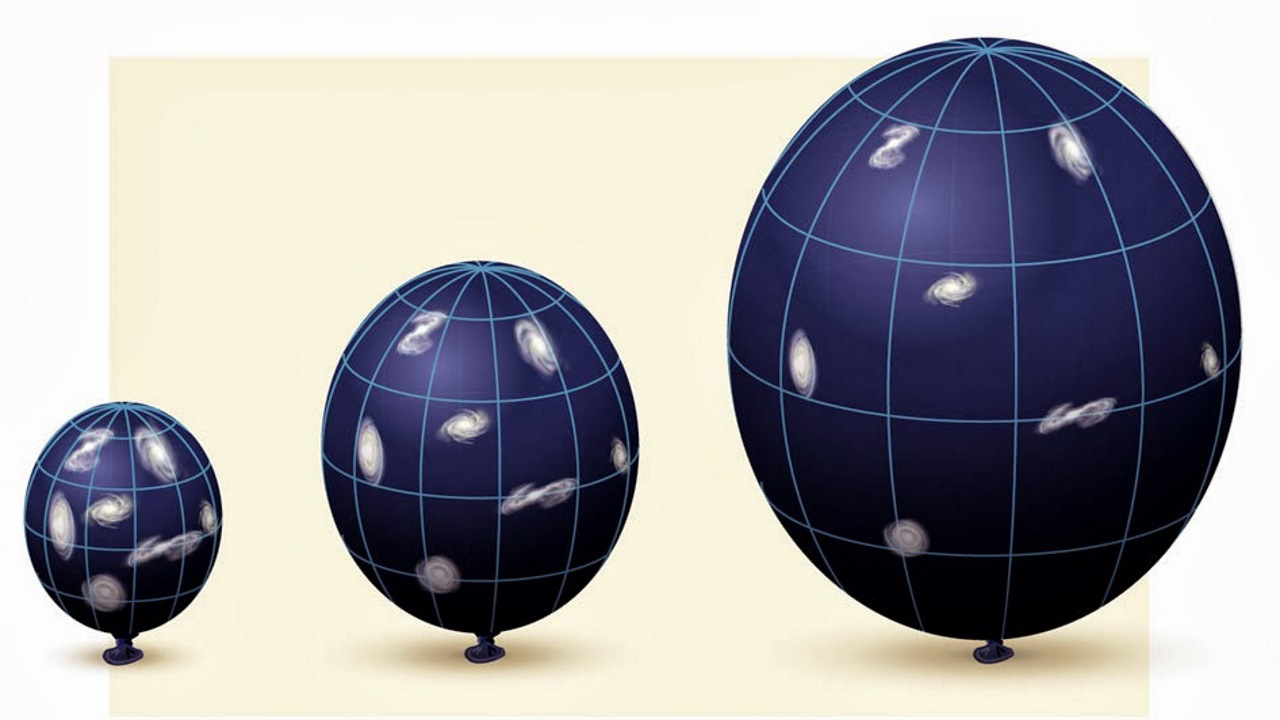
\includegraphics[scale=0.3]{Figures/universe-expansion.jpg}
\end{figure}
\end{frame}

%---------------------------------------------------------

\begin{frame}{Lyman $\alpha$ emission line}
A Ly$\alpha$ photon is emitted with a $\lambda= 1215.67 \AA$.  
\begin{figure}
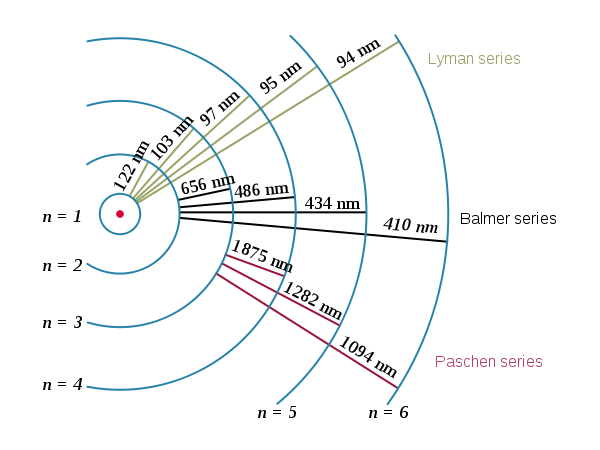
\includegraphics[scale=0.4]{Figures/Hydrogen_transitions.png}
\end{figure}
\end{frame}


%--------------------------------------------------------

\begin{frame}
\begin{figure}
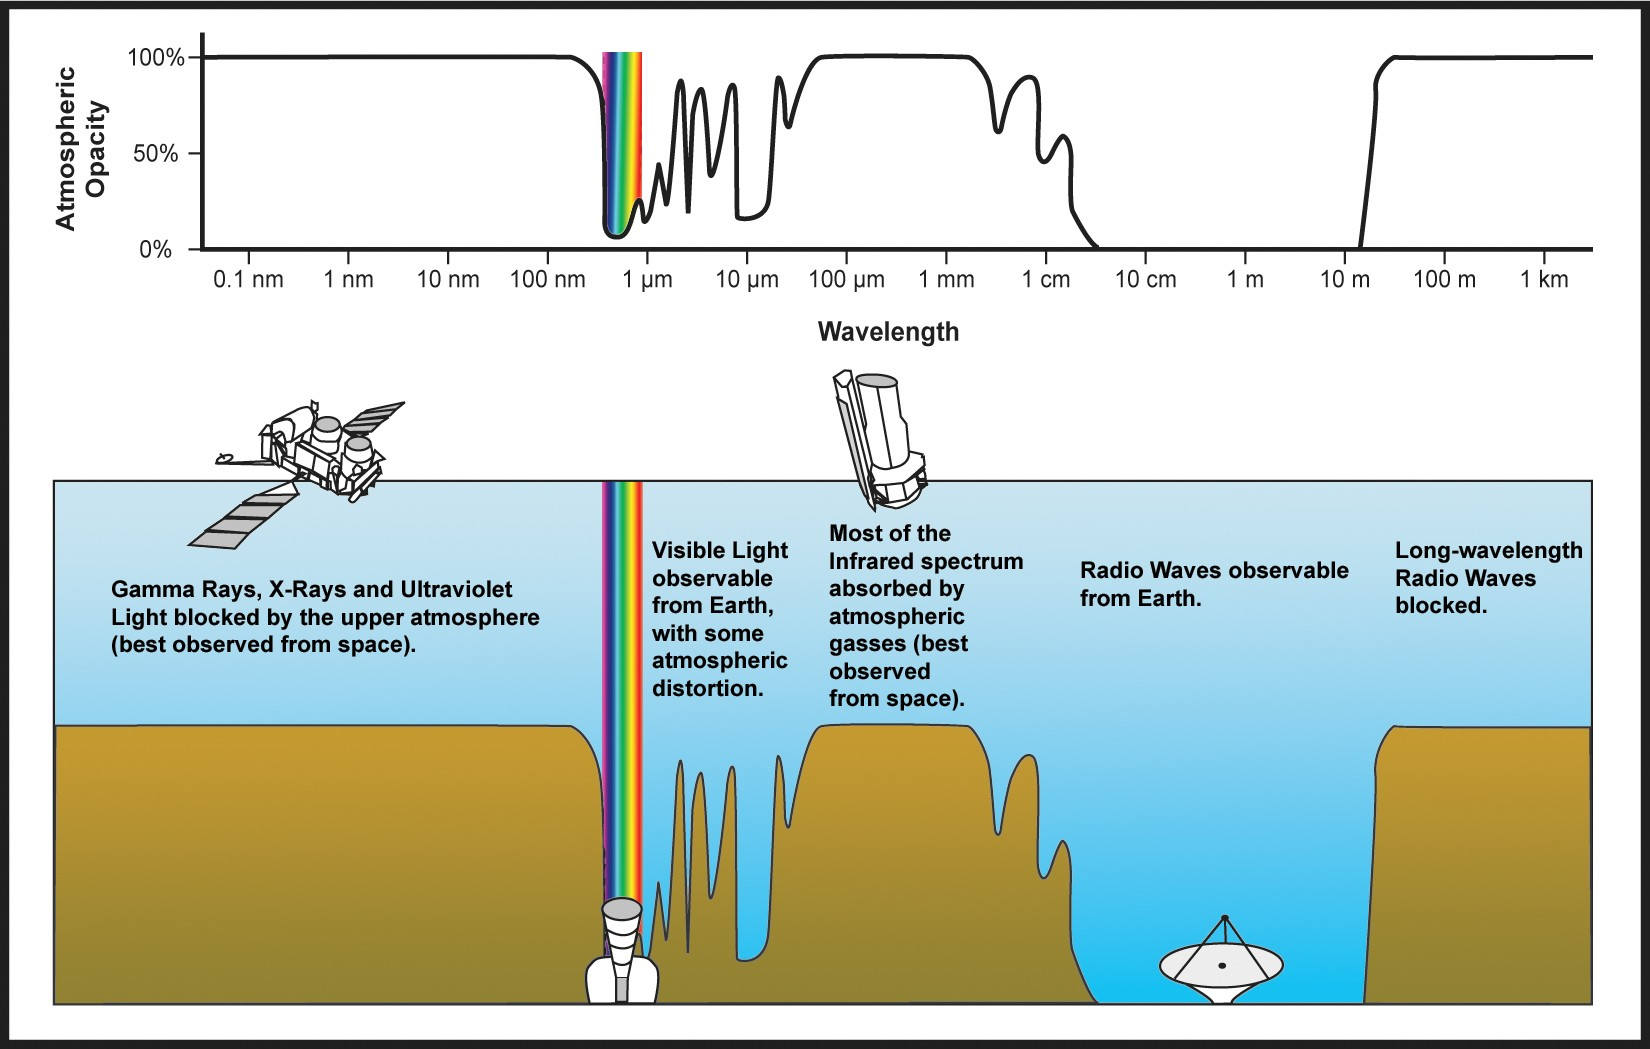
\includegraphics[scale=0.4]{Figures/AtmosphericEM.jpg}
\end{figure}
\end{frame}

%---------------------------------------------------------

\begin{frame}{Radiative Transfer code}
a
\end{frame}

%---------------------------------------------------------

\begin{frame}{Dust:}

\end{frame}

\begin{frame}{Simulated spectra}

\end{frame}

\end{document}
